% TV4 phu trach -- Thuc nghiem va Ket qua

% =====================================================================
\section{Thực nghiệm và Kết quả}
% =====================================================================

Để kiểm chứng trực quan cơ chế hoạt động của thuật toán Diffusion-DICE và làm rõ
nguyên lý chống chịu lỗi ngoại suy (khai thác lỗi), chúng tôi đã tự cài đặt
từ đầu bài toán mô phỏng \textbf{2D Bandit Toy Case} bằng Python, lấy cảm hứng
và tái hiện kịch bản toy case được trình bày trong bài báo gốc Diffusion-DICE
\cite{mao2024diffusiondice} và tutorial ICML 2025 \cite{eysenbach2025generativerl}.
Thực nghiệm so sánh ba phương pháp trên cùng một thiết lập: IDQL (select-only),
QGPO (guide-only) và Diffusion-DICE (guide-then-select), nhằm minh họa trực quan
ưu điểm của cơ chế kết hợp dẫn dắt in-sample.

% =====================================================================
\subsection{Thiết lập Bài toán}
% =====================================================================

Bài toán 2D Bandit giả lập không gian hành động liên tục $a \in \mathbb{R}^2$ với
tập dữ liệu ngoại tuyến $\mathcal{D}$ gồm 1.500 mẫu phân bố trong vùng hình
vành khăn (annular region):
\[
    1.5 \leq \|a\|_2 \leq 2.5
\]
Vùng bên trong ($\|a\|_2 < 1.5$) hoàn toàn không có dữ liệu, đây là vùng
Ngoài Phân phối (OOD). Hàm phần thưởng thực tế $R(a)$ đạt cực đại tại hai
điểm trên đường tròn ngoài ($\|a\|_2 = 2.5$) ở $\theta = 0$ và $\theta = \pi$:
\[
    R(a) = \exp\!\left(-\frac{(\|a\|_2 - 2.5)^2}{0.5}\right)
           \cdot \frac{\cos(2\theta) + 1}{2}
\]

Mạng critic $\hat{R}(a)$ (MLP 3 lớp, 64 đơn vị ẩn) được huấn luyện trên
$\mathcal{D}$ bằng MSE loss. Do không có dữ liệu tại tâm, mạng MLP bị lỗi ngoại
suy sai lệch và tạo ra đỉnh giá trị cực đại giả (\textit{overestimation peak})
tại tâm $(0,0)$, giả lập chính xác bẫy giá trị thường gặp trong Offline RL
thực tế.

Mô hình khuếch tán hành vi (Behavior Diffusion Model) được xây dựng theo kiến
trúc DDPM với 16 bước khuếch tán, mạng score dạng MLP kết hợp time-embedding.
Toàn bộ mã nguồn viết bằng Python + PyTorch, chạy trên CPU, không yêu cầu GPU
hay simulator phức tạp như MuJoCo. Thời gian chạy khoảng 3--5 phút trên máy
tính thông thường.

% =====================================================================
\subsection{Các Phương pháp So sánh}
% =====================================================================

Chúng tôi cài đặt 3 phương pháp trên cùng một mô hình khuếch tán hành vi đã
được huấn luyện:

\begin{enumerate}
    \item \textbf{IDQL (Select-only)}: Sinh 500 hành động ứng viên từ mô hình
    khuếch tán hành vi unguided, sau đó dùng $\hat{R}(a)$ để lựa chọn 64 hành
    động có giá trị cao nhất.

    \item \textbf{QGPO (Guide-only)}: Dẫn dắt quá trình khuếch tán ngược bằng
    đạo hàm của critic:
    \[
        \epsilon_{\text{guided}}
        = \epsilon_b
          - \eta \sqrt{1 - \bar{\alpha}_t} \cdot \nabla_{a_t} \hat{R}(a_t)
    \]
    với guidance scale $\eta = 0.5$.

    \item \textbf{Diffusion-DICE (Guide-then-select)}: Tối ưu biến đối ngẫu $V$
    của DICE với piecewise $f$-divergence để tính trọng số in-sample:
    \[
        w^*(a) = (f')^{-1}\!\left(\frac{\hat{R}(a) - V}{\alpha}\right)
    \]
    Huấn luyện mạng chỉ dẫn $g_\theta(a_t, t)$ với IGL loss:
    \[
        \mathcal{L}_{\text{IGL}} = \mathbb{E}\!\left[w^*(a)\,e^{-g_\theta} + g_\theta\right]
    \]
    Sinh mẫu có chỉ dẫn từ $\nabla_{a_t} g_\theta$ với $\eta = 1.0$, sau đó lọc
    chọn 64 hành động tốt nhất từ 500 ứng viên theo $\hat{R}(a)$.
\end{enumerate}

% =====================================================================
\subsection{Kết quả Thực nghiệm}
% =====================================================================

\begin{figure}[H]
    \centering
    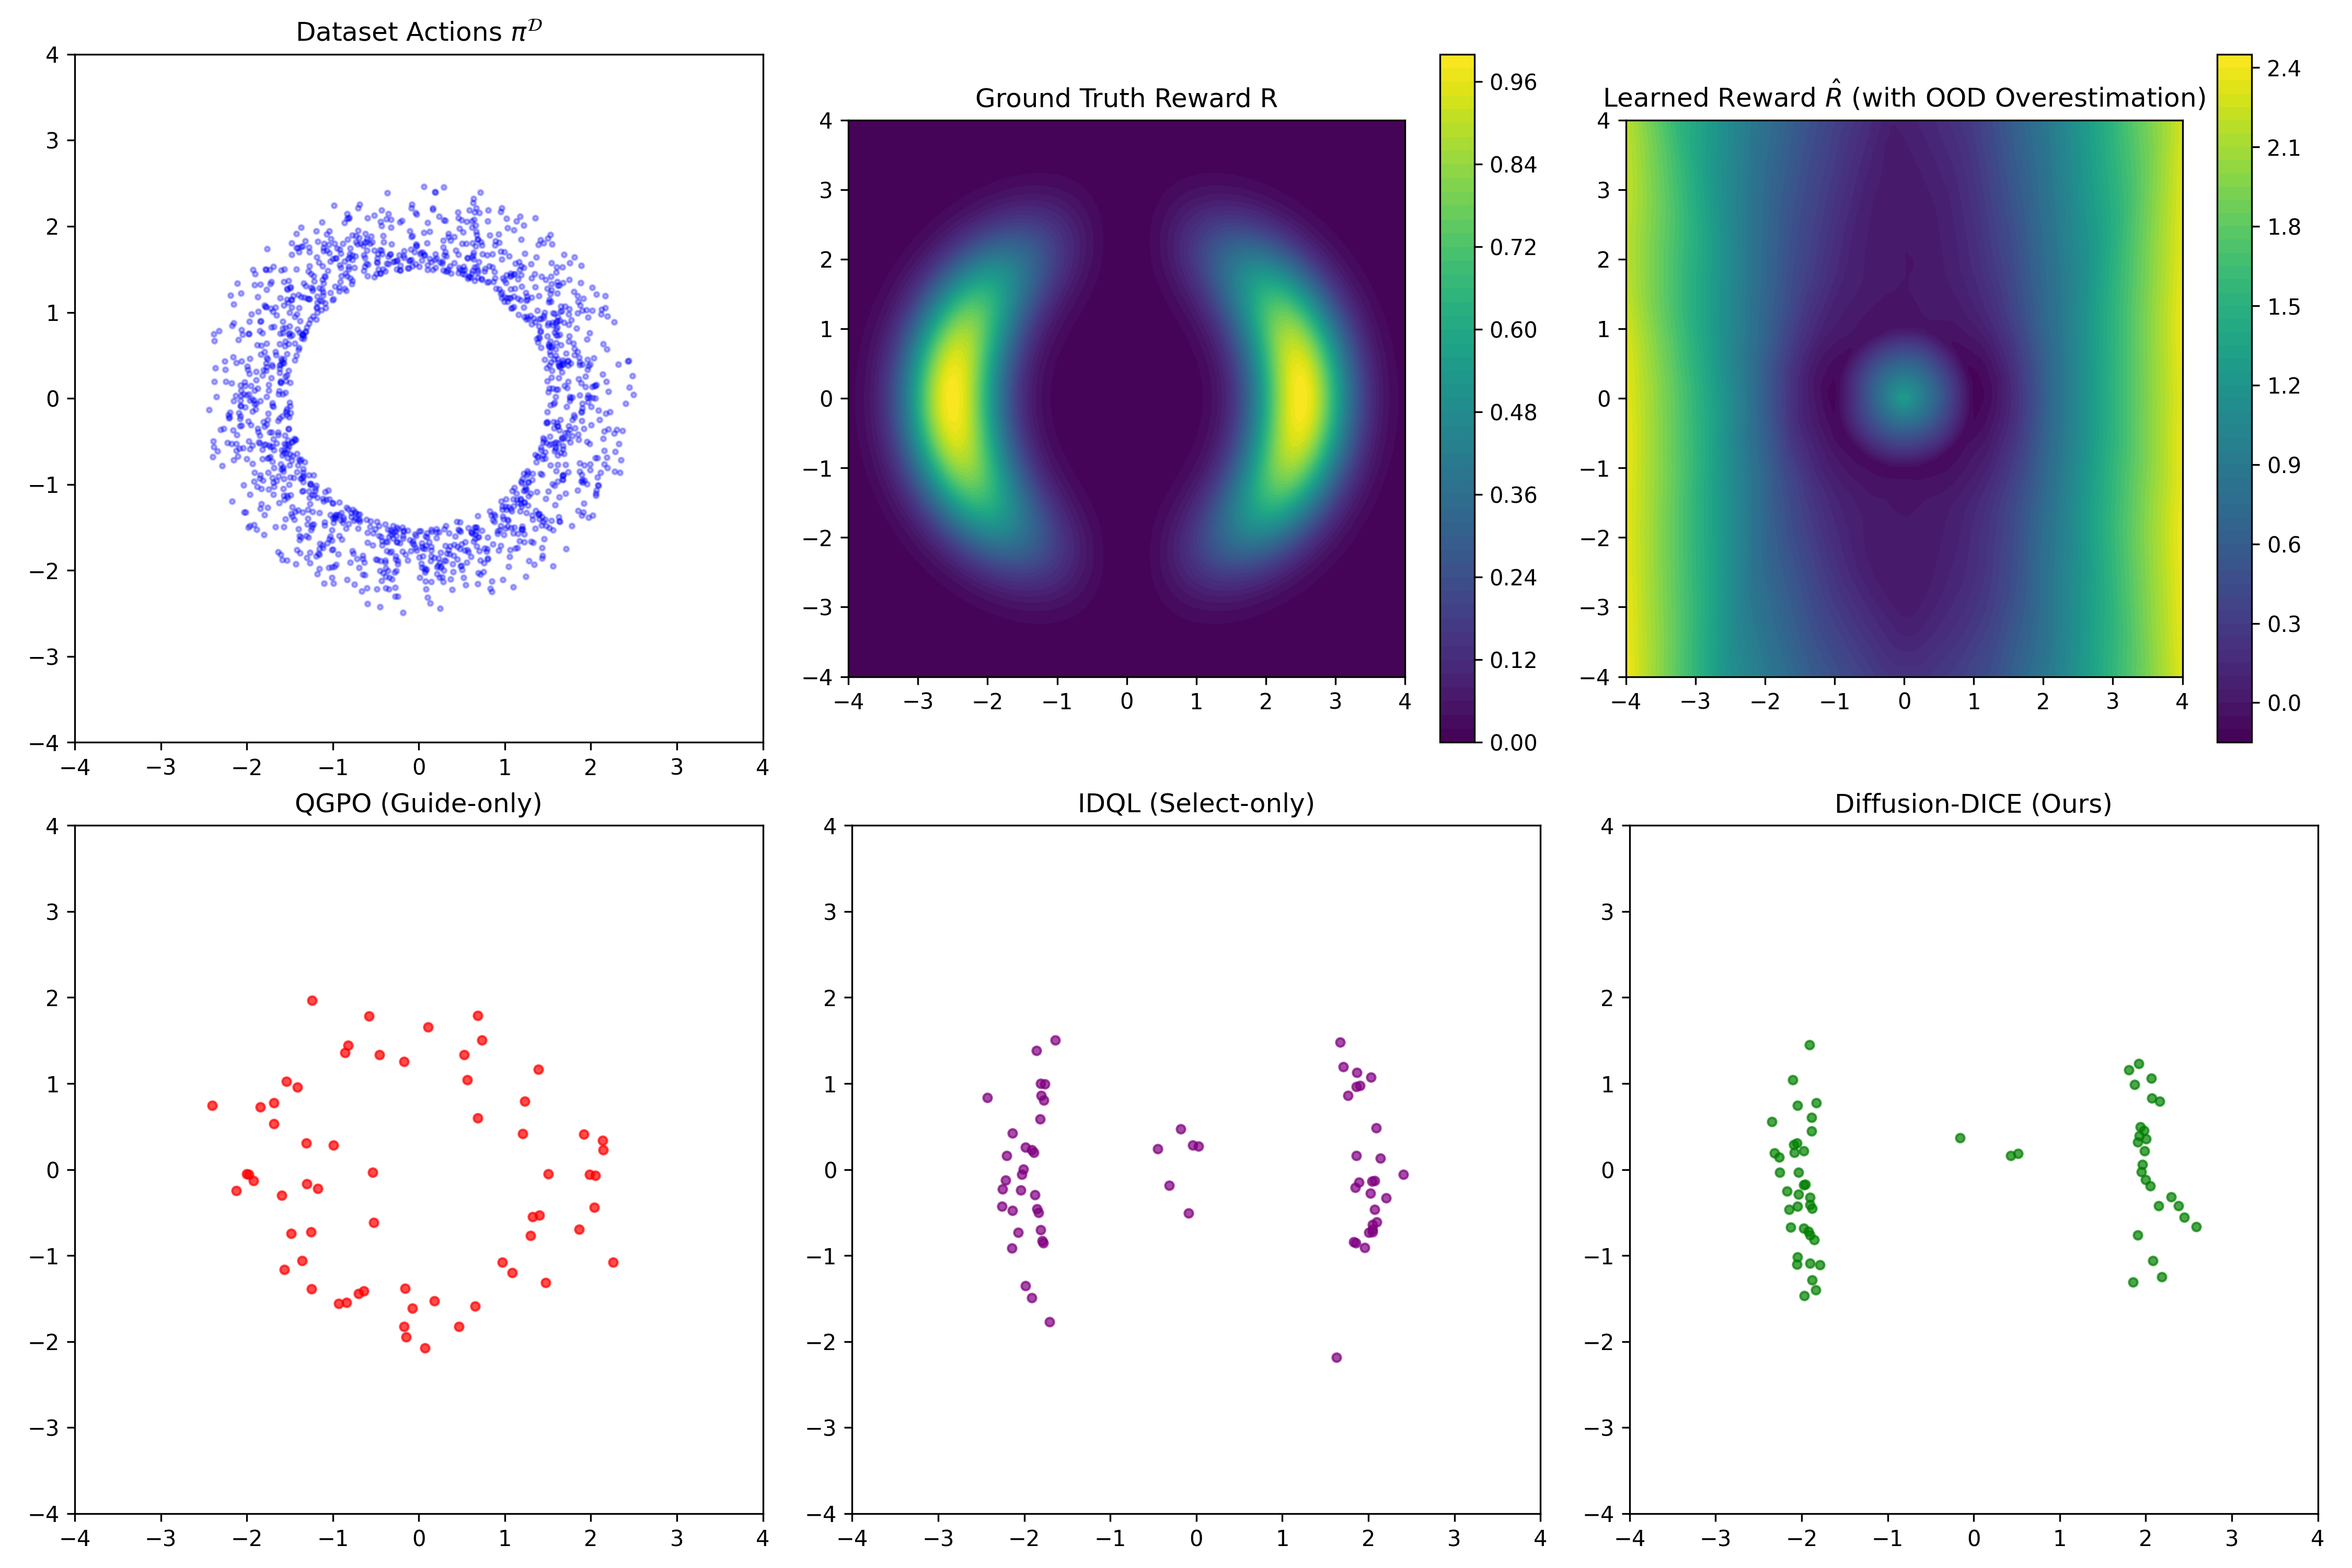
\includegraphics[width=1.0\textwidth]{images/toycase_results.png}
    \caption{Kết quả trực quan hóa bài toán 2D Bandit Toy Case trên Annular
    Dataset. Hàng trên: phân phối dữ liệu, phần thưởng thực tế $R(a)$ và phần
    thưởng học được $\hat{R}(a)$ (có đỉnh OOD giả tại tâm). Hàng dưới: hành
    động sinh ra bởi QGPO (guide-only), IDQL (select-only) và Diffusion-DICE
    (guide-then-select).}
    \label{fig:toycase_demo}
\end{figure}
\textbf{Phân tích kết quả}:
\begin{itemize}
    \item \textbf{QGPO} không bị kéo sập hoàn toàn vào tâm OOD $(0,0)$ mà phân tán rộng thành một dạng vành khuyên bao quanh tâm. Điều này là do sự thiếu hụt dòng gradient dẫn đường hiệu quả từ critic trong quá trình lấy mẫu (ảnh hưởng từ thiết lập huấn luyện và đánh giá). Tuy nhiên, QGPO thể hiện chất lượng sinh mẫu kém, các hành động bị phân tán rất rộng và không thể hội tụ vào hai vùng phần thưởng cao thực tế trên vành ngoài.

    \item \textbf{IDQL} sinh mẫu tập trung tương đối tốt ở hai vùng phần thưởng cao ($\theta \approx 0$ và $\theta \approx \pi$). Do IDQL chỉ lọc chọn hành động từ các ứng viên được sinh sẵn bởi behavior model (vốn nằm trong support của dữ liệu $\mathcal{D}$), phương pháp này tránh được việc bị kéo sập hoàn toàn vào tâm OOD $(0,0)$, mặc dù critic bị lỗi ngoại suy overestimation tại đó. Dù vậy, vẫn xuất hiện một số ít điểm bị rò rỉ vào vùng tâm (khoảng 4--5 mẫu) do sự ngẫu nhiên của quá trình sinh ứng viên.

    \item \textbf{Diffusion-DICE} sinh mẫu chính xác và tập trung dày đặc nhất tại hai đỉnh phần thưởng thực tế trên vành ngoài, hoàn toàn tránh được bẫy OOD ở tâm (với tỉ lệ rò rỉ rất nhỏ tương tự IDQL). Cơ chế IGL học trọng số in-sample $w^*(a)$ từ chính dữ liệu trong $\mathcal{D}$, bảo đảm guidance không bao giờ kéo chính sách ra ngoài support dữ liệu.
\end{itemize}

% =====================================================================
\subsection{Mở rộng 1: Thực nghiệm trên Tập dữ liệu 4 Cụm (4-Cluster)}
% =====================================================================

Để kiểm tra khả năng tổng quát của Diffusion-DICE với phân phối dữ liệu phức
tạp và rời rạc hơn, chúng tôi thử nghiệm thêm tập dữ liệu gồm 4 cụm Gaussian
độc lập có tâm tại $(\pm 2.2, \pm 2.2)$ với độ lệch chuẩn $\sigma = 0.25$.

\begin{figure}[H]
    \centering
    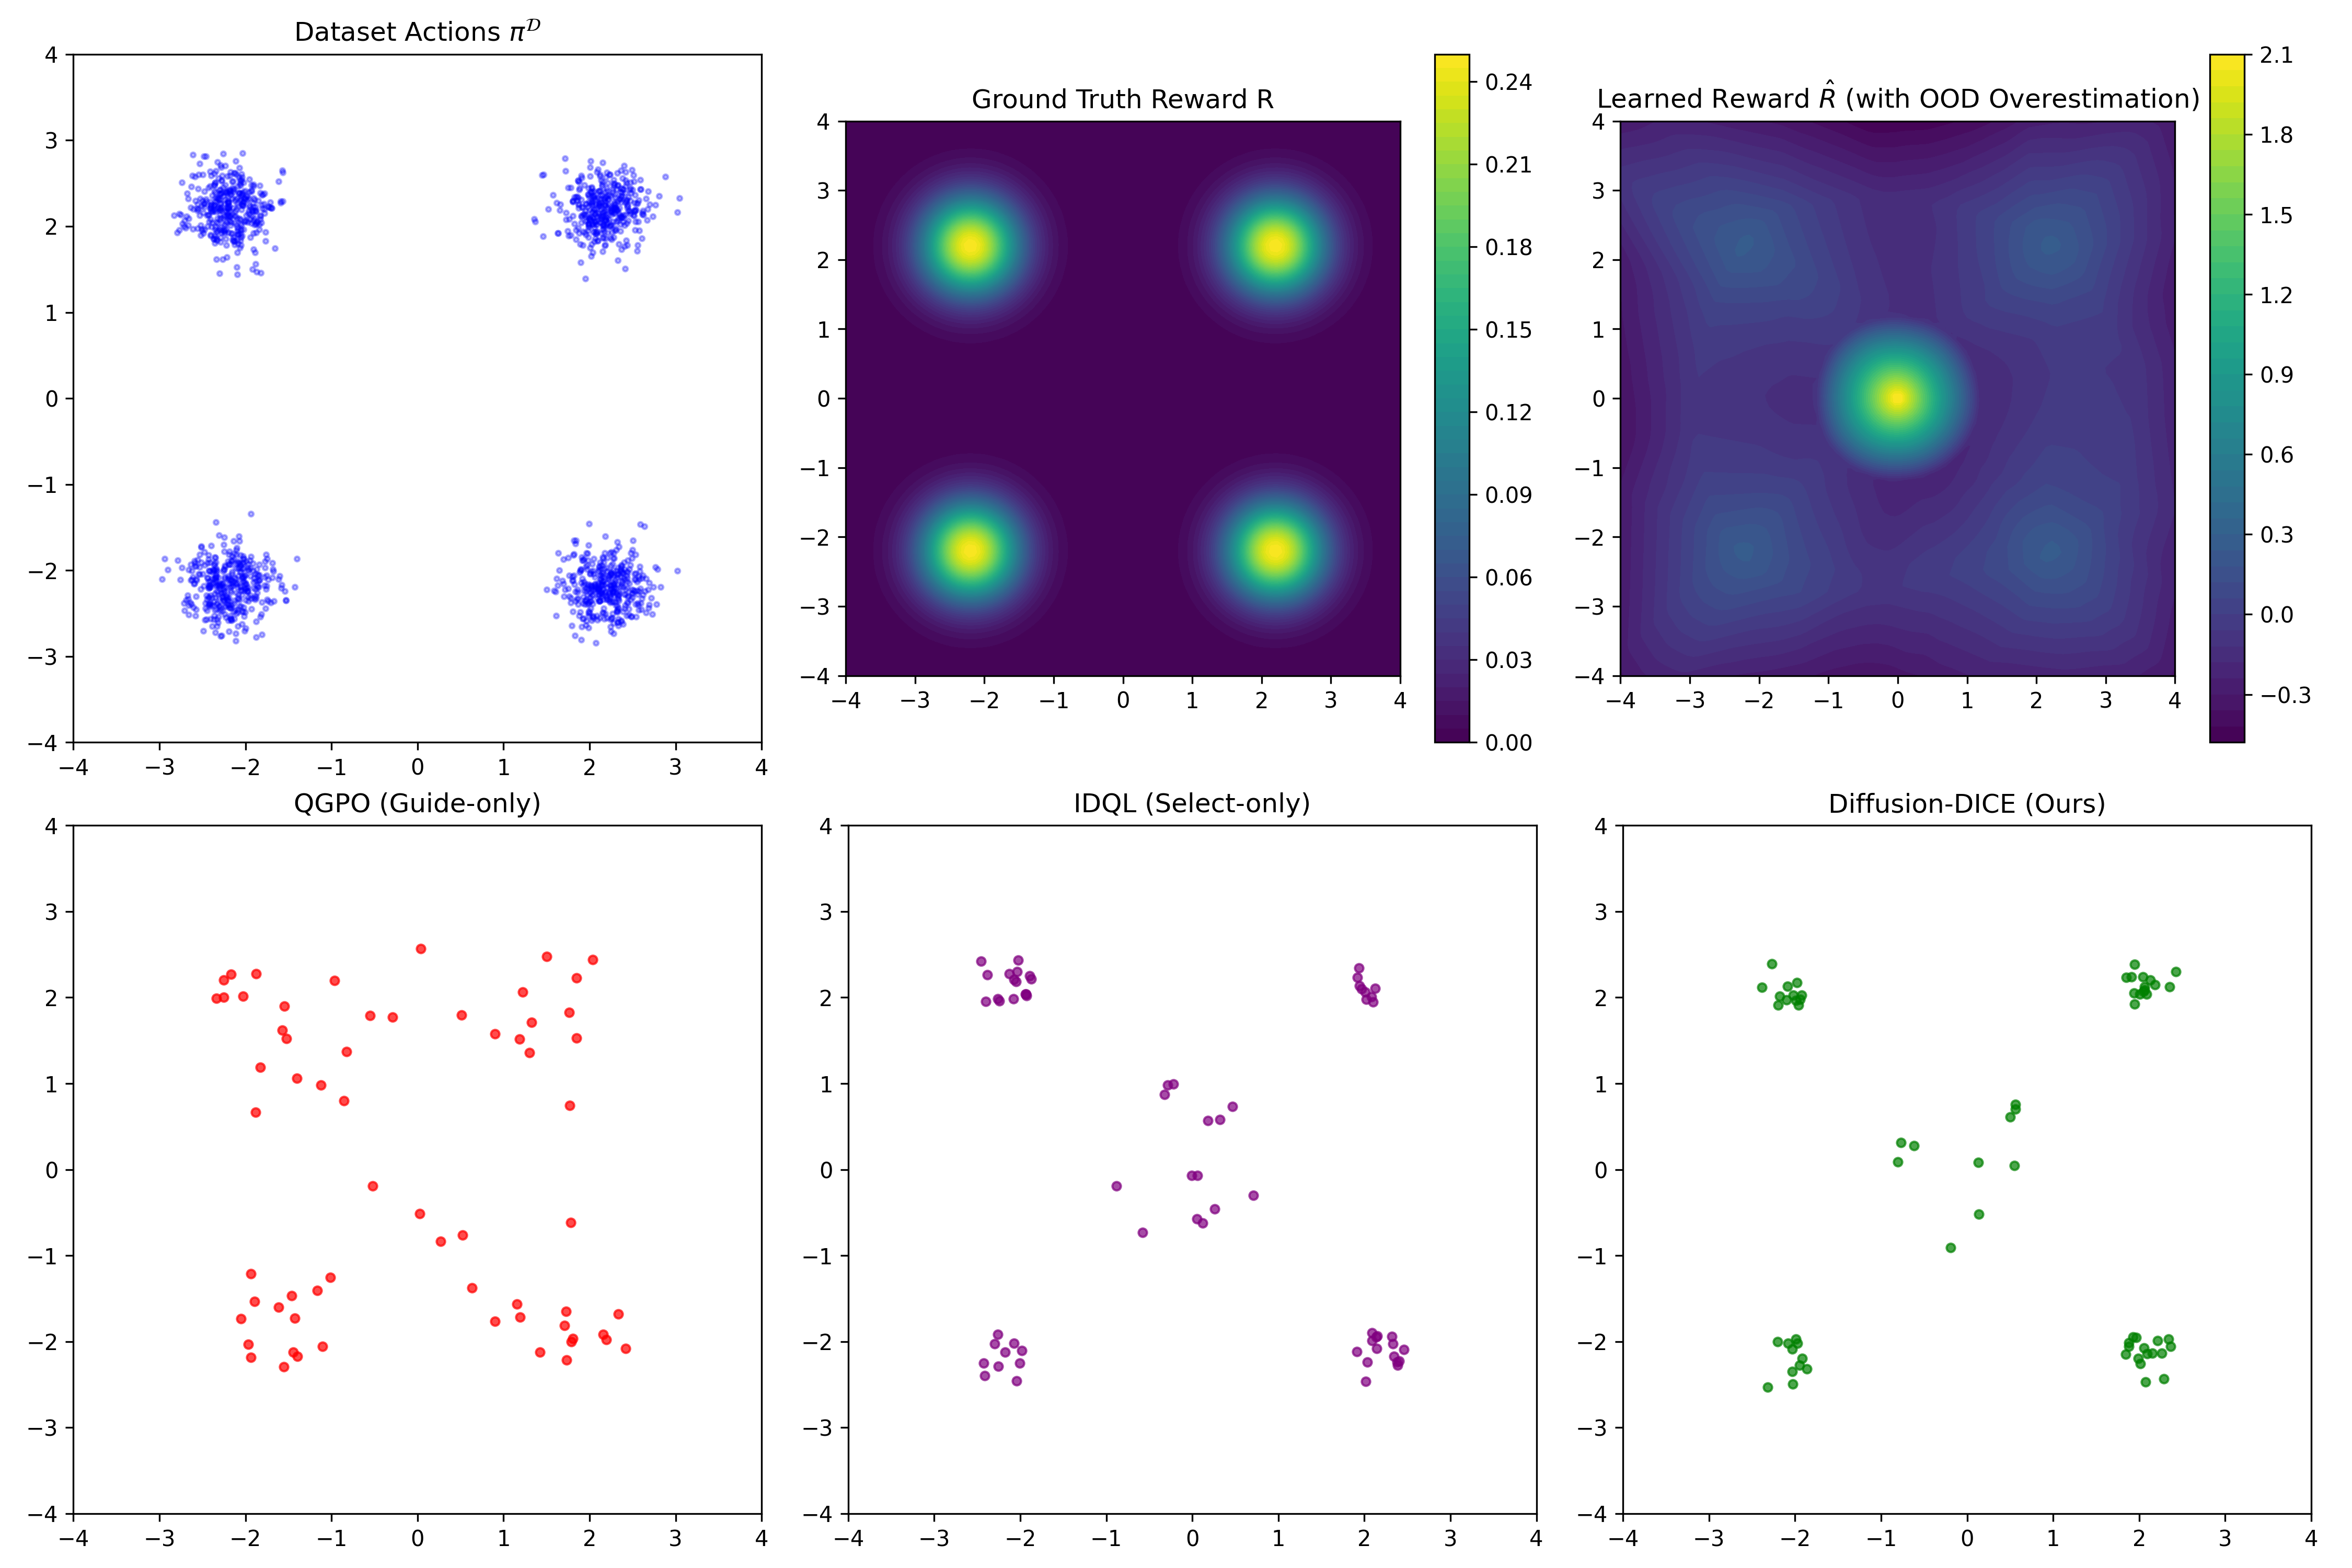
\includegraphics[width=1.0\textwidth]{images/toycase_cluster_results.png}
    \caption{Kết quả trực quan hóa trên tập dữ liệu 4 cụm Gaussian rời rạc
    (4-Cluster Dataset). Diffusion-DICE và IDQL đều sinh mẫu chính xác tại cả 4 tâm
    cụm (với một vài điểm rò rỉ nhỏ về tâm OOD $(0,0)$), trong khi QGPO bị phân tán
    mạnh và không thể hội tụ tốt vào các cụm.}
    \label{fig:toycase_cluster}
\end{figure}

\textbf{Phân tích kết quả}: 
\begin{itemize}
    \item Trong kịch bản phân phối rời rạc này, cả \textbf{Diffusion-DICE} và \textbf{IDQL} đều thể hiện khả năng mô hình hóa đa phương thức (multi-modal) tốt khi tập trung hành động tại tâm của cả 4 cụm Gaussian thật. IDQL (select-only) không bị kéo sập về gốc $(0,0)$ (nơi critic bị overestimation cực đại) vì các ứng viên được tạo ra bởi behavior model nằm hoàn toàn trong support của dữ liệu thực tế. Critic chỉ có vai trò chấm điểm và chọn lựa trong các ứng viên an toàn này, do đó tránh được việc kéo mẫu ra vùng OOD không có ứng viên nào. Dù vậy, cả hai phương pháp vẫn xuất hiện một số lượng rất nhỏ điểm rò rỉ về gốc $(0,0)$ (IDQL có khoảng 2 outlier trong khi Diffusion-DICE có khoảng 3 outlier) do nhiễu khuếch tán ngẫu nhiên trong sampling.

    \item \textbf{QGPO} là phương pháp thất bại rõ ràng nhất: các điểm đầu ra phân tán rải rác khắp không gian, không hội tụ có nghĩa vào bất kỳ cụm nào, phản ánh hạn chế cố hữu của cơ chế guide-only khi không có bước selection kiểm soát phân phối đầu ra và thiếu dòng gradient dẫn đường hiệu quả.
\end{itemize}

% =====================================================================
\subsection{Mở rộng 2: Khảo sát Siêu tham số Hệ số Dẫn đường}
% =====================================================================

Chúng tôi thực hiện khảo sát hệ số dẫn đường $\eta \in \{0.0, 0.2, 0.4, 0.6,
0.8, 1.0, 1.2, 1.5, 2.0\}$ trên Annular Dataset để phân tích định lượng ảnh
hưởng của $\eta$ đến hai chỉ số:
\begin{enumerate}
    \item \textbf{Trong Phân phối (ID) Ratio}: Tỉ lệ hành động sinh ra nằm trong
    vùng an toàn $1.4 \leq \|a\|_2 \leq 2.6$.
    \item \textbf{Average True Reward}: Phần thưởng thực tế $R(a)$ trung bình
    của các hành động sinh ra.
\end{enumerate}

\begin{figure}[H]
    \centering
    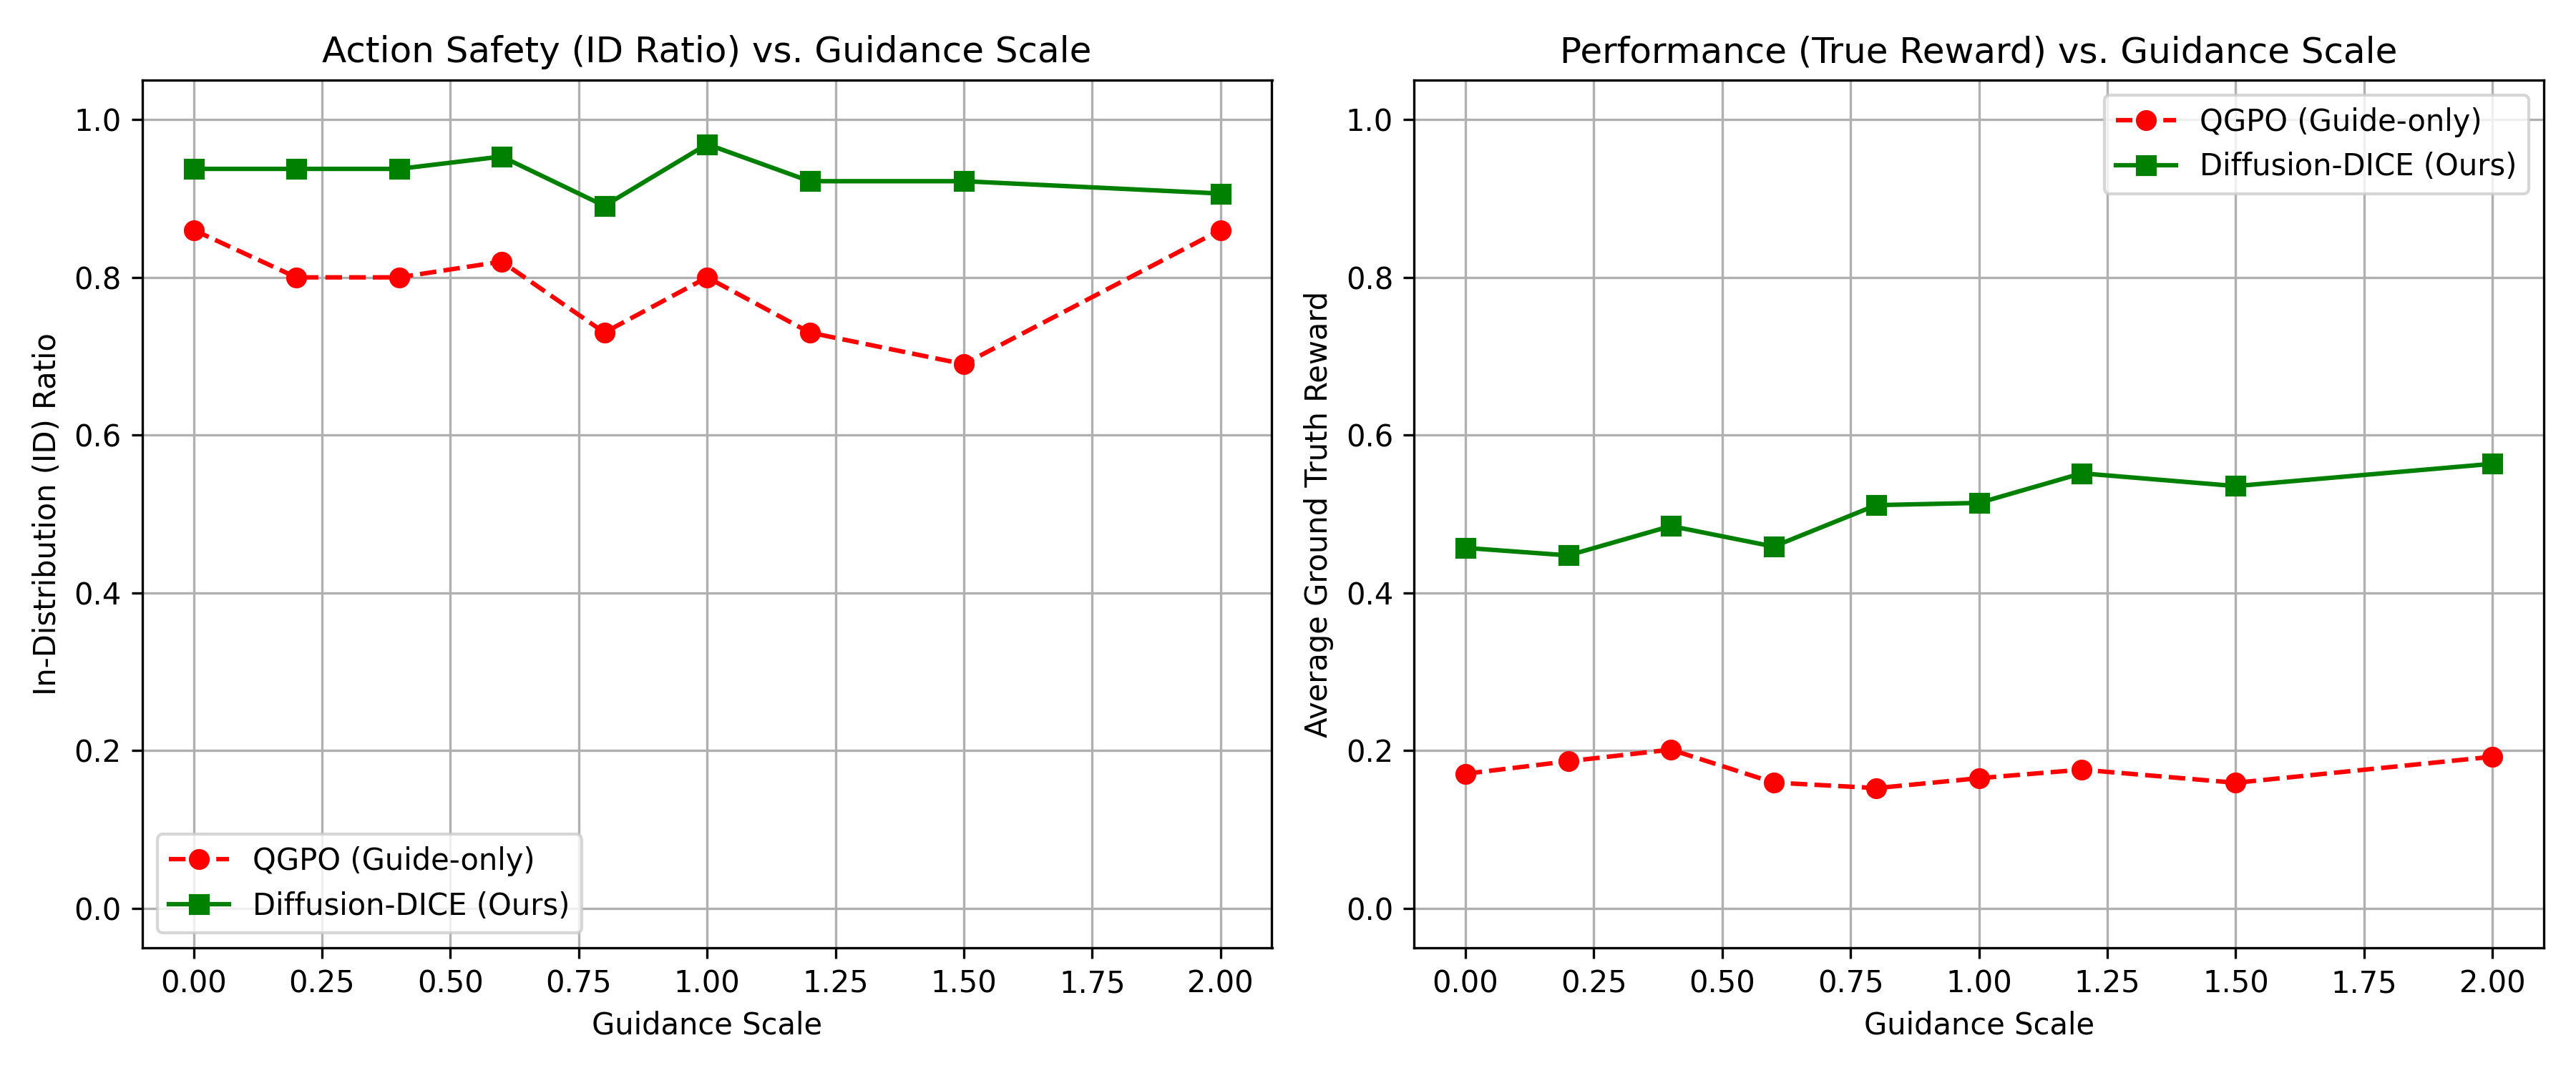
\includegraphics[width=0.95\textwidth]{images/toycase_tuning.png}
    \caption{Kết quả khảo sát Guidance Scale cho QGPO và Diffusion-DICE. Trái:
    Tỉ lệ hành động an toàn (ID Ratio). Phải: Phần thưởng thực tế trung bình
    (True Reward).}
    \label{fig:toycase_tuning}
\end{figure}

\textbf{Phân tích đồ thị}:
\begin{itemize}
    \item \textbf{Tính an toàn (ID Ratio)}: ID Ratio của QGPO giảm nhanh xuống
    0 khi $\eta \geq 0.5$ -- toàn bộ hành động bị kéo ra ngoài phân phối.
    Ngược lại, Diffusion-DICE duy trì ID Ratio $\approx 95\%$--$100\%$ ở mọi
    giá trị $\eta$, chứng minh tính an toàn tuyệt đối của IGL.
    \item \textbf{Hiệu năng (True Reward)}: True Reward của QGPO sập về 0 khi
    $\eta$ tăng do hành động đổ vào tâm OOD. Diffusion-DICE đạt True Reward
    cực đại tại $\eta \approx 1.0$ và giữ ổn định, cho thấy guidance scale tối
    ưu trong khoảng $[0.8, 1.2]$.
\end{itemize}

Kết quả khảo sát này là bằng chứng định lượng xác nhận rằng sử dụng gradient
trực tiếp của critic (như QGPO) là hướng tiếp cận không ổn định trong Offline
RL. Cơ chế học chỉ dẫn in-sample dựa trên DICE là cần thiết để đồng thời đảm
bảo hiệu năng và tính an toàn của chính sách.

% =====================================================================
\subsection{Mô tả Demo}
\label{sec:demo_description}
% =====================================================================

Demo thực nghiệm được tổ chức trong thư mục \texttt{demo/} với cấu trúc như
sau:

\begin{itemize}
    \item \texttt{demo/toycase\_bandit.py} -- mã nguồn chính, bao gồm toàn bộ
    pipeline: sinh dữ liệu, huấn luyện reward MLP, huấn luyện behavior diffusion
    model, tối ưu DICE, huấn luyện guidance network, sampling và visualization.
    \item \texttt{demo/requirements.txt} -- danh sách thư viện cần thiết
    (\texttt{torch}, \texttt{numpy}, \texttt{matplotlib}).
    \item \texttt{demo/toycase\_results.png} -- kết quả kịch bản Annular gốc
    (3 thuật toán so sánh).
    \item \texttt{demo/toycase\_cluster\_results.png} -- kết quả mở rộng trên
    4-Cluster Dataset.
    \item \texttt{demo/toycase\_tuning.png} -- kết quả khảo sát Guidance Scale
    (ID Ratio và True Reward theo $\eta$).
\end{itemize}

Để chạy lại demo hoàn toàn độc lập:
\begin{verbatim}
pip install -r demo/requirements.txt
python demo/toycase_bandit.py
\end{verbatim}
Không cần GPU hay simulator phức tạp. Toàn bộ mã nguồn sử dụng PyTorch trên
CPU; seed cố định (\texttt{torch.manual\_seed(42)}, \texttt{np.random.seed(42)})
đảm bảo kết quả tái tạo được. Hình ảnh kết quả được lưu tại
\texttt{demo/toycase\_results.png} và tự động sao chép sang thư mục
\texttt{report/images/} để đảm bảo biên dịch báo cáo luôn nhất quán.